\chapter{Medie di posizione}
\label{cha:mediePosizione}
\section{Moda}
\begin{definizione}[Moda]
Data una distribuzione di dati, la moda\index{Moda} è il valore che si presenta con più frequenza.
\end{definizione}
Poniamo di avere la seguente distribuzione di dati
\begin{center}
	\begin{tabular}{l*{5} {S[table-format=1.0]}}
		{$x_{i}=$}	&2  &7  &8  &3  &5 \\
		\midrule 
		{$n_{i}=$}	& 6 &8  & 5 & 10 & 2\\   
	\end{tabular}
\end{center}
\begin{figure}
	\centering
	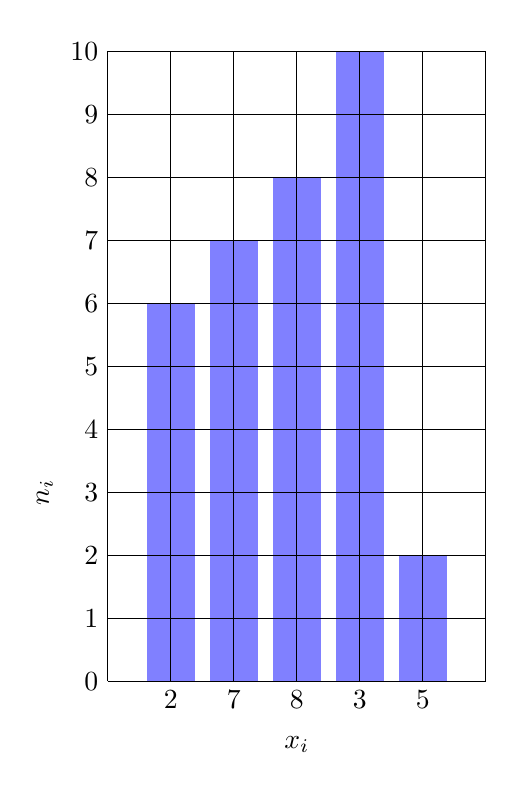
\begin{tikzpicture}[scale=0.8]
	\draw[line width=6mm,color=blue!50] plot[ycomb] coordinates{(1,6) (2,7) (3,8) (4,10)
		(5,2)};
	\draw (0,0) grid (6,10);
	\foreach \y in {0,1,...,10} \draw(0,\y)node[left]{\y};
	\foreach \n/\x in {5/5,3/4,8/3,7/2,2/1}
	\draw (\x,0) node [below] {\n};
	%\foreach \x in {1,2,...,10} \draw(\x,0)node[below]{\x};
	\draw (3,-1) node{$x_i$};
	\draw (-1,3) node[rotate=90]{$n_i$};
	\end{tikzpicture}
	\caption{Moda}
	\label{fig:Moda}
\end{figure}
Come si vede dal grafico~\vref{fig:Moda} il massimo numero di frequenze è per $n_i=10$ quindi la moda $M_o=3$. La moda non è sempre unica per esempio 
se abbiamo la seguente distribuzione di dati
\begin{center}
	\begin{tabular}{l*{5} {S[table-format=1.0]}}
		{$x_{i}=$}	&7  &3  &2  &4  &5 \\
		\midrule 
		{$n_{i}=$}	& 4 &2  & 3 & 4 & 2\\   
	\end{tabular}
\end{center}
Le frequenze massime sono due e sono per $n_i=4$ e le mode sono due $M_o=4$ e $M_o=4$ cioè si dice che le distribuzioni sono bimodali\index{Distrubuzione!bimodale} come appare nel grafico~\vref{fig:BiModale}
\begin{figure}
	\centering
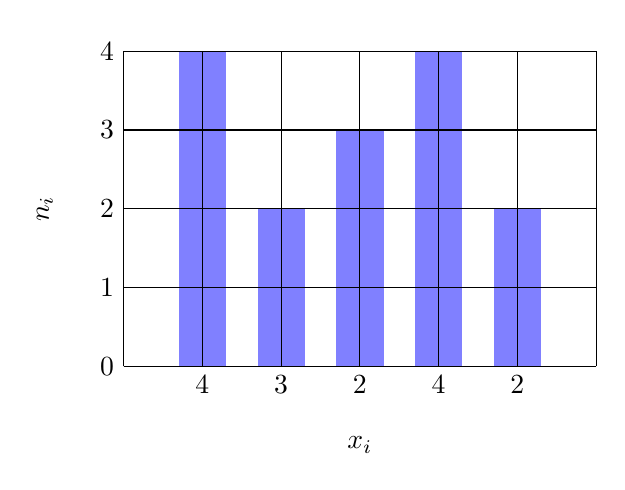
\begin{tikzpicture}%[scale=0.8]
\draw[line width=6mm,color=blue!50] plot[ycomb] coordinates{(1,4) (2,2) (3,3) (4,4)
	(5,2)};
\draw (0,0) grid (6,4);
\foreach \y in {0,1,...,4} \draw(0,\y)node[left]{\y};
\foreach \n/\x in {2/5,4/4,2/3,3/2,4/1}
\draw (\x,0) node [below] {\n};
%\foreach \x in {1,2,...,10} \draw(\x,0)node[below]{\x};
\draw (3,-1) node{$x_i$};
\draw (-1,2) node[rotate=90]{$n_i$};
\end{tikzpicture}
	\caption{Bimodale}
	\label{fig:BiModale}
\end{figure}
\subsection{Mediana}
\begin{definizione}[Mediana]
Dato un inseme ordinato di valori, la mediana\index{Mediana} che ha tanti dati che lo precedono quanti quelli che lo seguono.
\end{definizione}
Per determinare la mediana $M_e$ devo ordinare i dati in modo che $x_1\leq x_2\leq\cdots\leq x_n $. Avremo due casi il numero dei valori $n$ è dispari $k=\dfrac{n-1}{2}+1=\dfrac{n+1}{2}$. Con un esempio è più semplice: se ho undici valori e li ordino dal più piccolo al più grande, l'elemento di posto $ \dfrac{11+1}{2}=6$ è l'elemento che cerchiamo. Quel valore ha cinque elementi prima e cinque dopo. Se il numero totale  degli elementi è pari, non vi è un elemento centrale. In questo caso di pone per convenzione che se $k=\dfrac{n}{2}$ $M_e=\dfrac{x_k+x_{k+1}}{2}$